\chapter{Conversione AD e convertitori - parte II}

\begin{figure}[h]
    \centering
    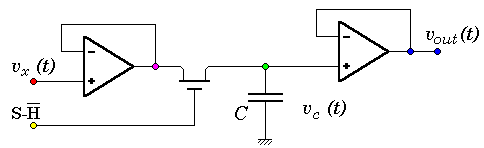
\includegraphics[scale = 1]{Sample And Hold e Track And Hold.png}
\end{figure}

\newpage 

\section{Fase 3: codifica}
\footnote{Slide della prof | SDME 3.Conversione AD e Convertitori - Parte II | pag 4 \\  
Appunti | 2025-03-25 | pag 2 - 3}

Dopo il campionamento e la quantizzazione, 
il segnale ha bisogno di essere codificato. \newline 

Per codifica si intende il processo che associa univocamente a ciascuno dei valori 
corrispondenti ai centri degli N intervalli in cui è stato suddiviso il campo di misura 
una "parola" (in questo caso) binaria a M bit. \newline 

È necessario che ciascuno degli N valori quantizzati disponga di una "sua" parola. \newline 

Siccome non ci devono essere codifiche doppie è richiesto che: 

{
    \Large 
    \begin{equation}
        N \le 2^{M}
    \end{equation}
}

La scelta ottimale della codifica va fatta rispetto al livello di tensione e dei dispositivi che devono rielaborare il segnale. \newline 

Questo corso non tratterà della scelta ottimale della codifica, 
bensì tratteremo esclusivamente della mappatura ottimale per la quantizzazione silenziata, 
essendo quella che garantisce reiezione al disturbo. \newline 

\newpage 

\section{Mappatura ottimale per la quantizzazione silenziata}
\footnote{Slide della prof | SDME 3.Conversione AD e Convertitori - Parte II | pag 5 - 8 \\  
Appunti | 2025-03-25 | pag 3}

Avendo un campo di misura simmetrico, cioè da $-E_c$ e $+E_c$, 
per ottenere una quantizzazione silenziata bisogna avere un numero dispari  di intervalli. \newline 

Consideriamo quindi: 

{ 
    \Large 
    \begin{equation}
        N = 2^{M} - 1
    \end{equation}
}

Siccome si considera un numero di N che è minore di $2^{M}$, 
l'incertezza di quantizzazione sarà maggiore. \newline 

L'errore di quantizzazione e sarà: 

{
    \Large 
    \begin{equation}
        e = \frac{2 E_c}{2^{M} -1}
    \end{equation}
}

Se consideriamo N dispari e una quantizzazione silenziata, 
i livelli di quantizzazioni graficati saranno del tipo: 

\begin{figure}[h]
    \centering
    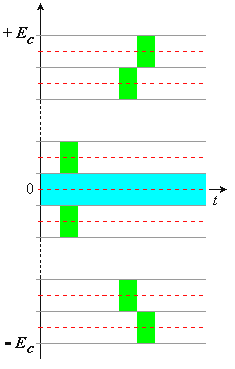
\includegraphics[scale = 0.8]{Quantizzazione silenziata con N livelli dispari.png}
\end{figure}

Avere N dispari complicherebbe le operazioni in binario, 
che invece sarebbero semplici se N fosse una potenza di 2. \newline 

Si parte da una quantizzazione non silenziata, e poi si traslano tutti gli intervalli in basso di mezzo livello. \newline 

Con questo shift, dalla figura precedente, otteniamo la seguente figura: 

\begin{figure}[h]
    \centering
    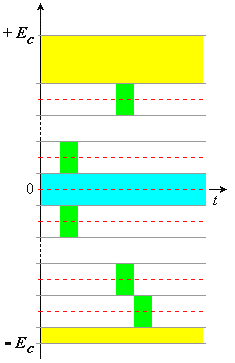
\includegraphics[scale = 0.8]{Quantizzazione silenziata con N livelli dispari shiftata.png}
\end{figure}

\newpage 

Si ottiene un intervallo centrato nello zero e i rimanenti intervalli di quantizzazione ottenuti 
dividendo il campo di misura da $-E_c$ a $+E_c$ in $2^{M}$ parti. \newline 

Disponendo di M bit per la codifica, avremo che: 

{
    \Large 
    \begin{equation}
        \begin{cases}
            N \leq 2^{M}
            \\
            N = 2^{M} 
            \\  
            e = \frac{2 E_c}{N}
        \end{cases}
    \end{equation}
}

Ma così facendo, abbiamo creato due intervalli (quelli evidenziati in giallo) 
che non andremo ad usare e presentano ampiezze diverse perchè non sono uniformi 
rispetto agli altri livelli di quantizzazione. \newline 

Di seguito la stessa figura, ma con maggiori considerazioni scritte a lezione: 

\begin{figure}[h]
    \centering
    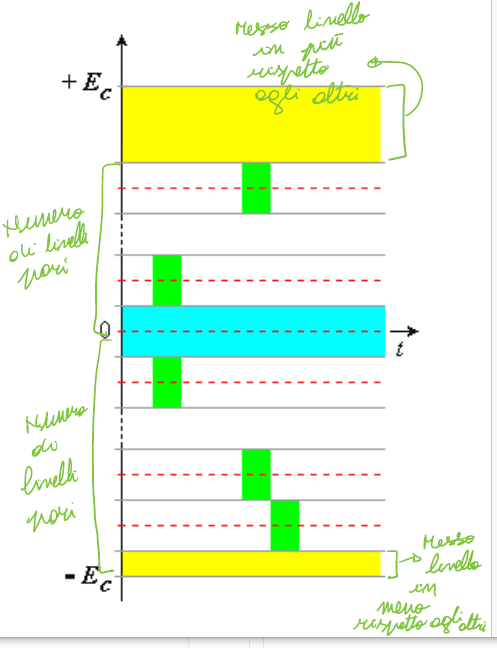
\includegraphics[scale = 0.5]{Quantizzazione silenziata con N livelli dispari shiftata con appunti pag 6.png}
\end{figure}

Di seguito la tecnica di quantizzazione effettivamente usata negli ADC commerciali. \newline 

I due intervalli segnati in giallo, apparentemente "persi", possono essere usati per segnalare due condizioni di errore: 

\begin{itemize}
    \item condizione di overflow, quando il segnale di ingresso arriva al limite superiore del campo di misura (cioè l'intervallo giallo di $+E_c$) 
    \item condizione di underflow, quando il segnale di ingresso ha valore troppo basso, prossimo al limite inferiore del campo di misura (cioè l'intervallo giallo di $-E_c$)
\end{itemize}

In tutti gli altri intervalli non in giallo, essendo equi-spaziati e costanti, l'incertezza sarà costante in ciascun intervallo. \newline 

Supponendo un esempio con i seguenti valori: 

{
    \Large 
    \begin{equation}
        \begin{split}
            M &= 8 
            \\ 
            &\downarrow 
            \\
            N &= 2^{M} 
            \\ 
            &= 2^{8}
            \\
            &= 256
        \end{split}
    \end{equation}
}

Questo significa che il livello minimo 0000 0000 e quello massimo 1111 1111 saranno usati per segnalare 
le condizioni di, rispettivamente, underflow e overflow. \newline 

I rimanenti 254 livelli, saranno utilizzati per codificare il segnale. \newline 

\newpage 

\section{La conversione A/D reale}
\footnote{Slide della prof | SDME 3.Conversione AD e Convertitori - Parte II | pag 9 \\  
Appunti | 2025-03-25 | pag 4} 

Dopo aver spiegato cosa significa svolgere un campionamento, 
di seguito sarà presentato un esempio di architettura di campionatore. \newline 

Il campionatore che analizzeremo è quello del Sample and Hold, Track and Hold. \newline 

Da un punto di vista ideale, possiamo rappresentarlo così: 

\begin{figure}[h]
    \centering
    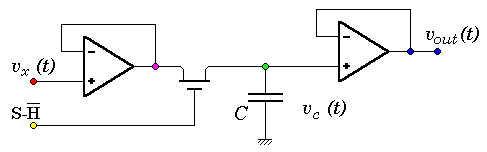
\includegraphics[scale = 0.8]{Sample and Hold e Track and Hold ideale.png}
\end{figure}

I componenti principali di un "Sample and Hold" (compattato come S \& H) sono: 

\begin{itemize}
    \item due OpAmp connessi come inseguitore di tensione, quindi il circuito presenterà un guadagno unitario 
    \item un MOS-FET che opera come interruttore 
    \item un condensatore C che opera come memoria 
\end{itemize}

La scelta del valore del condensatore C sarà cruciale per il S \& H. \newline 

\newpage 

\section{Sample and hold: funzionamento ideale}

\subsection{Ipotesi di componenti ideali} 
\footnote{Slide della prof | SDME 3.Conversione AD e Convertitori - Parte II | pag 10 \\  
Appunti | 2025-03-25 | pag 2 - 4} 

Ipotizziamo i componenti dell'S \& H ideali, cioè: 

\begin{itemize}
    \item gli OpAmp avranno impedenza infinita in ingresso e impedenza nulla in uscita 
    \item il mosfet sarà a perfetta conduzione o perfetta interdizione perchè si comporterà da interruttore 
    \item il condensatore è una capacità ideale in cui la la carica che si immagazzina non si dissipa, cioè non ci sono correnti di fuga, e si scarica istantaneamente
\end{itemize}

Siccome consideriamo un Mos-FET come interruttore, il circuito da: 

\begin{figure}[h]
    \centering
    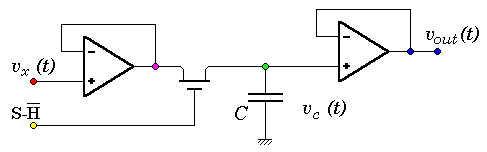
\includegraphics[scale = 0.8]{Sample and Hold e Track and Hold ideale.png}
\end{figure}

passerà a: 

\begin{figure}[h]
    \centering
    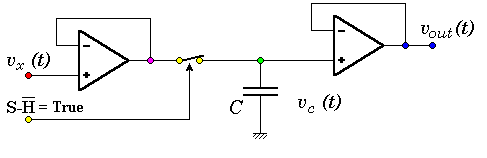
\includegraphics[scale = 0.8]{Sample and Hold e Track and Hold ideale con interruttore.png}
\end{figure}

\newpage 

\subsection{Interruttore chiuso} 
\footnote{Slide della prof | SDME 3.Conversione AD e Convertitori - Parte II | pag 11 - 14\\  
Appunti | 2025-03-25 | pag 4 - 5} 

Consideriamo il caso in cui l'interruttore venga chiuso, grazie al segnale alto di Sample 
dal pin $S-\overline{H}$. \newline 

Il circuito diventerà: 

\begin{figure}[h]
    \centering
    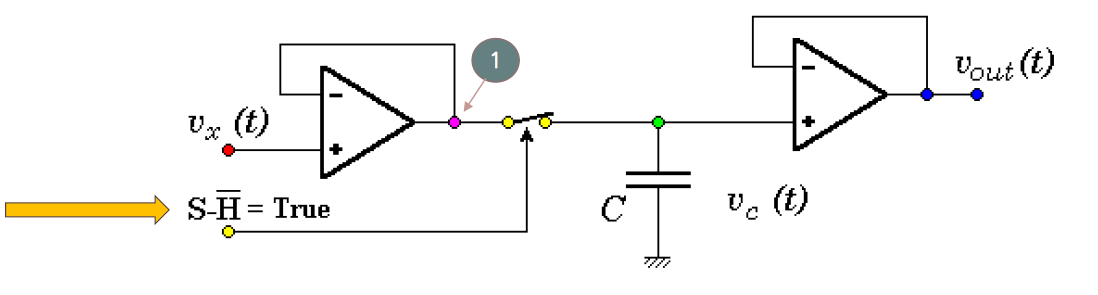
\includegraphics[scale = 0.5]{Sample and Hold e Track and Hold ideale con interruttore abbassato con note.png}
\end{figure}

Se l'interruttore è chiuso, essendo l'AmpOp in configurazione inseguitore, 
la tensione che si ha nel nodo rosso $v_{x} (t)$ la si avrà anche nel nodo rosa (segnato con il cerchio 1). \newline 

Essendo l'interruttore, cioè il Mos-fet, chiuso, la tensione $v_{x} (t)$ va a caricare il condensatore C, 
il quale si porta ad una tensione $v_c$ uguale a $v_x$ (nodo verde). \newline 

Il secondo OpAmp a destra ha ingresso $v_c$ (nodo verde), è in configurazione non invertente, 
quindi $v_{out} (t)$ (nodo blu) ha la stessa tensione di $v_c (t)$. \newline 

Ipotizzando che in questo momento $v_x(t)$ abbia l'andamento di una rampa, possiamo graficare $v_x (t)$, che è uguale a $v_{out} (t)$ 
e il segnale di enable del $S-H$ come: 

\begin{figure}[h]
    \centering
    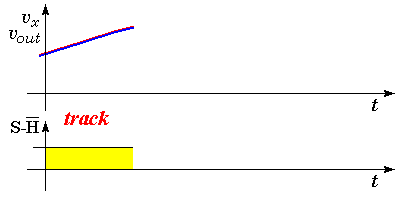
\includegraphics[scale = 0.8]{Segnale ingresso e di uscita del S&H e del segnale di enable.png}
\end{figure}

Ad un istante di tempo arbitrario, il sistema viene interdetto: 
portando al livello basso il segnale che pilota l'interruttore, si apre:  

\begin{figure}[h]
    \centering
    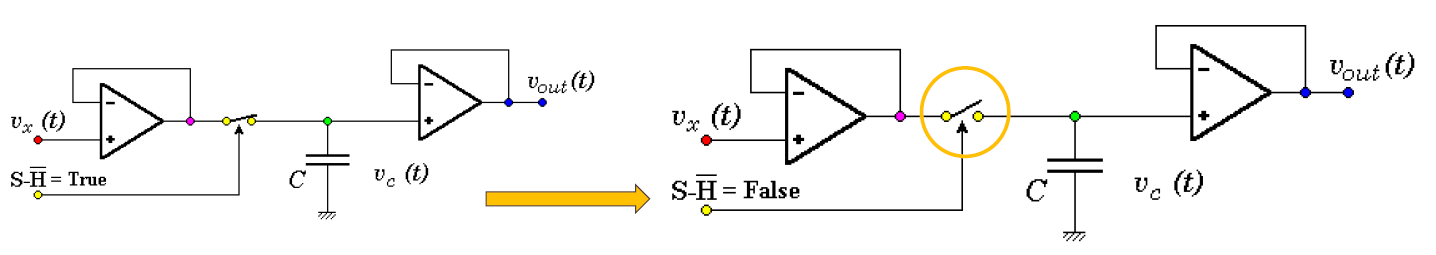
\includegraphics[scale = 0.4]{Da track a hold nell'S&H interruttore.png}
\end{figure}

Il circuito a sinistra si definisce come "S \& H in track-mode" (track perchè l'andamento di $v_{out} (t)$ è uguale a quello di $v_x (t)$), 
il circuito a destra, cioè con l'interruttore alto, si definisce come "S \& H in hold-mode" (hold perchè si cercherà di mantenere $v_{out} (t)$ costante uguale a $v_x (t)$ nell'istante $t_0$ 
dove $t_0$ è il momento in cui si alza l'interruttore). \newline 

La tensione di ingresso può variare arbitrariamente, ma, poiché l'interruttore è aperto, 
la variazione della tensione $v_x$ non raggiunge la seconda parte del circuito, 
cioè la parte del circuito a destra dell'interruttore. \newline 

Le tempistiche di track e hold devono rispettare le condizioni di Shannon-Nyquist. \newline 

Ora che l'interruttore è aperto, l'AmpOp a destra non seguirà più la tensione di $v_x (t)$, 
bensì quella del condensatore $v_c (t)$. \newline 

Siccome si considera un condensatore C ideale, le cariche accumulate sulla capacità non possono "sfuggire" perchè: 

\begin{itemize}
    \item verso sinistra il circuito è aperto (resistenza infinita) 
    \item verso destra, l'impedenza di ingresso dell'OpAmp ideale è infinita (concetto della massa virtuale spiegato precedentemente) 
    \item le armature sono perfettamente isolate, quindi le cariche restano nel condensatore e mantengono la tensione $v_c (t)$ ad un valore costante, che aveva nell'istante $t_0$ in cui l'interruttore è stato aperto
\end{itemize}

Ripetendo che anche l'AmpOp a destra è in configurazione non invertente, durante la fase di hold, $v_{out} (t)$ sarà uguale a $v_c (t)$ 
che, idealmente, rimane costante. \newline 

Utilizzando le figure: 

\begin{figure}[h]
    \centering
    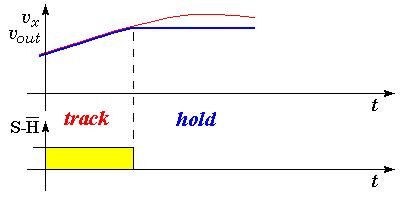
\includegraphics[scale = 0.7]{hold time per S&H.png}
\end{figure}

in cui: 

\begin{itemize}
    \item la funzione blu è l'andamento di $v_{out}$ 
    \item la funzione rossa è l'andamento di $v_x$, che nell'istante di hold può variare arbitrariamente 
    \item il segnale $S - \overline{H}$ è a livello basso, quindi avviene la fase di hold
\end{itemize}

Aprendo l'interruttore all'istante di campionamento, 
mantengo il segnale di uscita al valore che il segnale di ingresso aveva proprio in quell'istante e do il tempo ai circuiti successivi 
all'S \& H di effettuare quantizzazione e codifica. \newline 

Una volta che si è effettuato quantizzazione e codifica, bisogna ripetere i processi svolti precedentemente, 
ma questa volta per un nuovo istante di tempo. \newline 

Quindi, dalla fase di hold, bisogna ripassare alla fase di track (che dall'inglese significa inseguimento). \newline 

Graficando i grafici di $v_x$, $v_{out}$ e dell'enable pin $S - \overline{H}$: 

\begin{figure}[h]
    \centering
    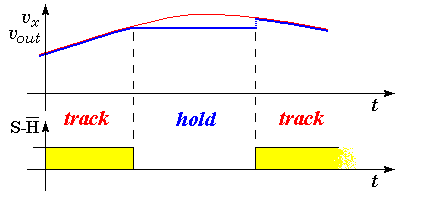
\includegraphics[scale = 0.8]{track-hold-track nell'S&H.png}
\end{figure}

Come si nota dal grafico di $v_{out}$ (funzione in blu), idealmente tra il tempo di hold al tempo di track, 
la tensione $v_{out}$ diventa uguale a quella di $v_x$. \newline 

Quindi ritorniamo al caso precedente dove, nel periodo di track: 

{
    \Large 
    \begin{equation}
        v_x = v_{out} = v_c
    \end{equation}
}

La tensione ai capi del condensatore si porta rapidamente (idealmente lo fa in maniera istantanea) 
al livello della tensione $v_x$ erogato in uscita dall'inseguitore (primo OpAmp) e altrettanto rapidamente la tensione $v_{out}$ 
si porta al suo livello, eseguendo così una nuova fase di track. \newline 

A un certo punto $t_1$ arriva un nuovo istante di campionamento, l'interruttore si apre di nuovo e si segue la fase 
di mantenimento (hold) e il processo hold-track e track-hold si ripete. \newline 

Tutto questo processo, da un punto di vista ideale, è molto semplice perchè i componenti si comportano istantaneamente e idealmente. \newline 

\newpage 


\section{Sample and Hold: funzionamento reale} 
\footnote{Slide della prof | SDME 3.Conversione AD e Convertitori - Parte II | pag 15 - 29 } 

\subsection{L'acquisition time sull'S\&H reale} 
\footnote{Slide della prof | SDME 3.Conversione AD e Convertitori - Parte II | pag 15 - 16 \\  
Appunti | 2025-03-25 | pag 5 - 6} 

Nel S \& H ideale avevamo visto che tra la fase di hold-track, 
$v_{out}$ (funzione blu) insegue subito la tensione di ingresso $v_x$ (funzione rossa) come in figura: 


\begin{figure}[h]
    \centering
    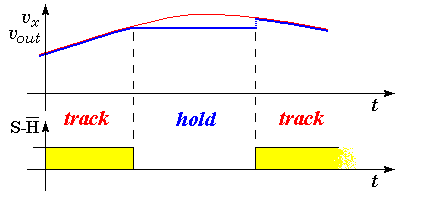
\includegraphics[scale = 0.8]{track-hold-track nell'S&H.png}
\end{figure}

MA, nella realtà non avviene ciò. \newline 

\begin{tcolorbox}
    Nella realtà non esiste tutto subito e infinito. Altra regola aurea
\end{tcolorbox}

Nella realtà, il grafico delle tensioni del circuito saranno le seguenti: 

\begin{figure}[h]
    \centering
    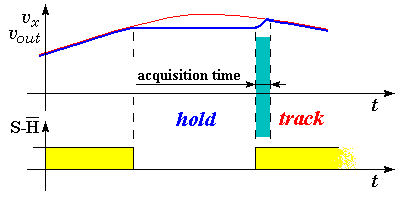
\includegraphics[scale = 0.8]{tensioni in un S&H reale.png}
\end{figure}

Il nuovo elemento è l'acquisition time. \newline 

L'acquisition time è quel tempo che, nel mondo reale, 
è la somma tra il tempo che serve al primo Amp-Op per riportarsi al livello di $v_x$ 
dovuto alla resistenza non nulla di uscita dell'inseguitore definito come transitorio di carica 
e la resistenza non nulla del MOS-FET. \newline 

L'acquisition time può essere visto anche come un tempo di ritardo tra l'istante in cui si attiva 
la fase di track e l'istante in cui la tensione $v_c (t)$ aggancia la $v_x$. \newline 

Essendo $v_c (t)$ la tensione ai capi di un condensatore, 
$v_c (t)$ sale con andamento esponenziale, in questo caso smorzato 
perchè, dopo l'acquisition time,  $v_c = v_x$. \newline 

Dall'elettrotecnica, la costante di tempo con cui la tensione cresce dipende dal valore della capacità C scelta. \newline 

Quindi, per questo motivo, se si vuole mantenere basso l'acquisition time, bisogna avere un valore di C più basso possibile. \newline 

Non si può avviare una nuova fase di campionamento fino a che la tensione ai capi del condensatore non ha agganciato la $v_x$: 
questa fase si definisce come acquisition time esaurito. \newline 

Con tutte queste considerazioni, rispetto al mondo ideale, l'intervallo di campionamento 
non sarà uguale al tempo di hold, bensì alla somma tra il tempo di hold e l'acquisition time. \newline 

In formule: 

{
    \Large 
    \begin{equation}
        \begin{split}
            t_\text{campionamento ideale} &\le t_\text{campionamento reale}
            \\
            &\downarrow
            \\
            t_{hold} &\le t_{hold} + t_\text{acquisition time}
        \end{split}
    \end{equation}
}

Si può osservare che parte del valore del tempo di campionamento $T_c$, 
dato dal teorema di Shannon-Nyquist, dipende dalla rapidità dei circuiti di quantizzazione e codifica, 
e una parte dipende dal sample-and-hold. \newline 


\newpage 

\subsection{L'effetto delle ricombinazioni delle cariche sul S \& H reale} 
\footnote{Slide della prof | SDME 3.Conversione AD e Convertitori - Parte II | pag 17 - 19 \\  
Appunti | 2025-03-25 | pag 6} 

Consideriamo il caso del circuito S \& H ideale: 

\begin{figure}[h]
    \centering
    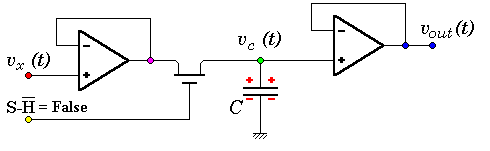
\includegraphics[scale = 0.8]{S&H ideale con cariche del condensatore.png}
\end{figure}

Considerando ideale i componenti, il condensatore C accumula le cariche (indicate di rosso) ai capi delle sue armature per sempre. \newline

Considerando invece il circuito S \& H reale, possiamo modellarlo in questa maniera: 

\begin{figure}[h]
    \centering
    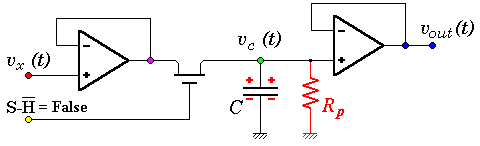
\includegraphics[scale = 1]{S&H reale con cariche del condensatore.png}
\end{figure}

Rispetto al circuito ideale, è presente anche una resistenza parassita $R_p$. \newline 

\begin{tcolorbox}
    Piccola guida alla notazione utilizzata dalla prof: 
    \begin{itemize}
        \item $R_p$ con la R maiuscola si intende una resistenza parassita che, idealmente, dovrebbe essere la più grande possibile 
        \item $r_p$ con la r minuscola si intende una resistenza parassita che, idealmente, dovrebbe essere la più piccola possibile
    \end{itemize}
\end{tcolorbox}

Si modella questa resistenza parassita $R_p$ in parallelo al condensatore C per rappresentare il fenomeno delle ricombinazione delle cariche. \newline 

In questo caso, per ricombinazione delle cariche si intende che, se idealmente le cariche dovrebbero rimanere ai capi delle armature del condensatore C, 
nella realtà si disperdono nel circuito (e generalmente sotto forma di calore) per i seguenti motivi del mondo reale: 

\begin{itemize}
    \item l'impedenza di ingresso dell'OpAmp a destra di C è elevata ma non è infinita 
    \item l'isolamento tra le armature del condensatore C è elevato ma non è infinito 
    \item anche in interdizione, cioè quando il MOS-FET idealmente dovrebbe essere un interruttore aperto, nella realtà lascia passare una debolissima corrente
\end{itemize}


In fase di hold, le cariche del condensatore C, anziché rimanere sulle armature, 
passano da una armatura all'altra tramite la $R_p$, come mostrato nelle seguenti figure: 

\begin{figure}[h]
    \centering
    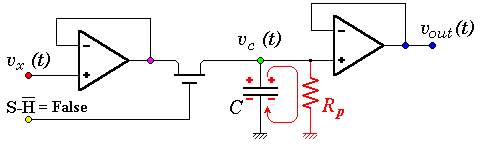
\includegraphics[scale = 1]{S&H reale con cariche del condensatore scarica 1.png}
    \\
    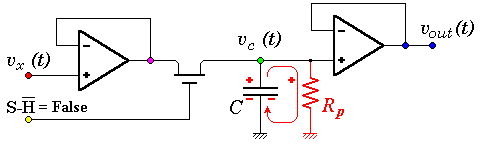
\includegraphics[scale = 1]{S&H reale con cariche del condensatore scarica 2.png}
    \\
    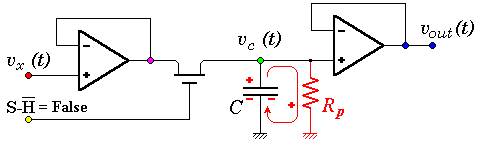
\includegraphics[scale = 1]{S&H reale con cariche del condensatore scarica 3.png}
    \\
    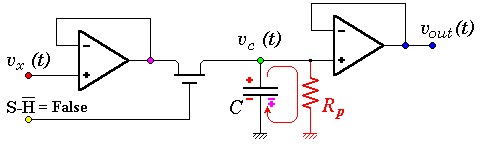
\includegraphics[scale = 1]{S&H reale con cariche del condensatore scarica 4.png}
\end{figure}

\newpage

quindi si ha la scarica del condensatore. \newline 

Dall'elettrotecnica e sapendo che in parallelo a C c'è una resistenza $R_p$, la tensione ai capi di C non resta costante, 
ma segue un esponenziale decrescente. \newline 

Da un punto di vista grafico, si passerà dal grafico delle tensioni del circuito ideale: 

\begin{figure}[h]
    \centering
    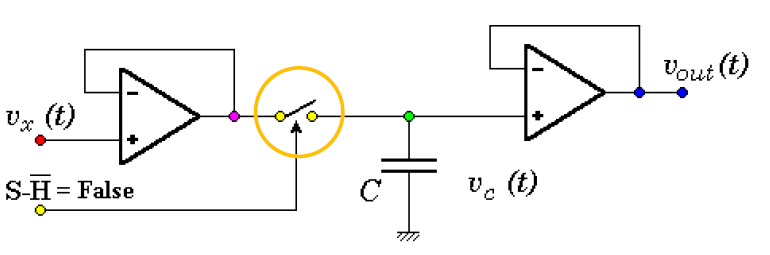
\includegraphics[scale = 0.4]{S&H ideale interruttore aperto.PNG}
    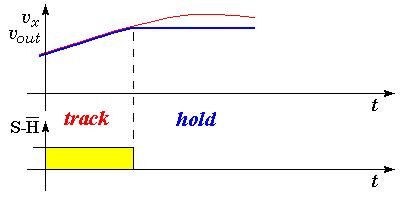
\includegraphics[scale = 0.6]{hold time per S&H.png}
\end{figure}

al grafico delle tensioni nel circuito reale: 

\begin{figure}[h]
    \centering
    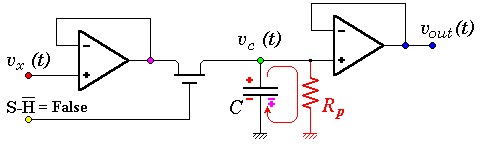
\includegraphics[scale = 1]{S&H reale con cariche del condensatore scarica 4.png}
    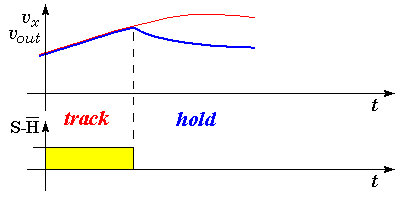
\includegraphics[scale = 1]{S&H reale tensioni hold time.png}
\end{figure}

Poiché tutte le impedenze che danno origine alla $R_p$ e che sono dovute alle non idealità dei componenti 
e anche alle anomalie delle giunzioni, non sono costanti, si preferisce (come al solito) semplificare la trattazione 
e considerare la scarica con andamento lineare anziché esponenziale decrescente. \newline 

Dall'elettrotecnica, si può stimare la pendenza della curva esponenziale come: 

{
    \Large 
    \begin{equation}
        \tau = RC
    \end{equation}
}

\newpage 

\subsection{Droop rate (velocità di discesa della tensione)} 
\footnote{Slide della prof | SDME 3.Conversione AD e Convertitori - Parte II | pag 20 - 21 \\  
Appunti | 2025-03-25 | pag 6 - 7} 

Come scritto precedentemente, piuttosto che calcolarci l'andamento esponenziale della scarica del condensatore, 
si cerca di linearizzarlo perchè è più semplice per i calcoli. \newline 

\begin{tcolorbox} 
    Linearizzare la pendenza della retta di $\tau = RC$ causa una sovrastima dell'entità della scarica, 
    ma sovrastimare è meglio perchè sicuramente funzionerà meglio il progetto
\end{tcolorbox}

Allora, dall'andamento esponenziale decrescente, si sceglierà di passere al seguente andamento lineare della tensione di $V_{out}$ e quindi di $V_c$. \newline 

Partendo dall'andamento esponenziale, calcoliamo l'angolo $\alpha$

\begin{figure}[h]
    \centering
    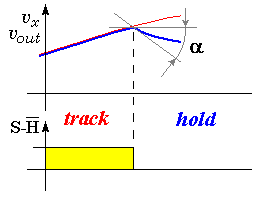
\includegraphics[scale = 1.5]{Droop rate nel S&H reale.png}
\end{figure}

Da $\alpha$ si calcola il droop rate come: 

{
    \Large 
    \begin{equation}
        \tan(\alpha) = \text{Droop rate}
    \end{equation}
}

Il droop rate esprime la pendenza della curva di scarica del condensatore nella fase iniziale. \newline 

Si considera che la scarica prosegua sempre con quella pendenza. \newline 

La tangente dell'angolo $\alpha$ è il droop rate, la velocità di discesa della tensione. \newline 

Il droop rate dipende dalla resistenza parassita $R_p$, che consente la ricombinazione delle cariche. \newline 

La corrente che passa sulla $R_p$ è legata alla tensione $v_c(t)$ e non alla capacità. \newline 

Se dovessi raddoppiare la capacità, la corrente si manterrebbe invariata perchè essa dipende da $v_c (t)$. \newline 

Allora, se io aumentassi la capacità del condensatore, la corrente circolante sulla $R_p$ rimarrebbe invariata, 
ma, si rallenterebbe molto il processo di diminuzione della tensione $v_c(t)$. \newline 

Nella realtà, la $R_p$ è una resistenza non lineare. \newline 

Aumentando C, si riduce il droop rate perchè aumentano il numero di cariche accumulate. \newline 

\newpage 

\subsection{Droop voltage} 
\footnote{Slide della prof | SDME 3.Conversione AD e Convertitori - Parte II | pag 22 - 23 \\  
Appunti | 2025-03-25 | pag 7} 

Aumentando la durata di fase di hold, aumenta il droop: spiegato diversamente, la tensione iniziale si riduce. \newline 

Il droop considerato accettabile negli ADC deve essere inferiore della metà dell'ampiezza dell'intervallo di quantizzazione perchè 
la tensione $v_{out}(t_0)$ deve rimanere nel bin (cestino) dell'intervallo di quantizzazione. \newline 

Le figure spiegano meglio il processo appena introdotto: 

\begin{figure}[h]
    \centering
    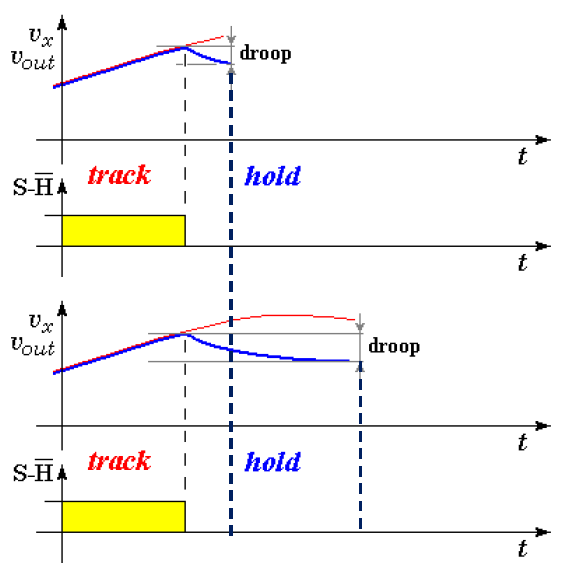
\includegraphics[scale = 1]{Scelta del droop rate negli ADC.png}
\end{figure}

Tipicamente, i costruttori di ADC mettono a disposizione un PIN sul quale collegare un condensatore 
col valore di capacità stabilito in funzione dei requisiti del progetto, quindi si ha fisicamente lo stesso S \& H 
ma per diversi tempi di track e hold. \newline 

Per la non linearità di $R_p$, si cerca di linearizzarlo con la seguente formula: 

{
    \Large 
    \begin{equation}
            \text{droop voltage} [t_0, t] = \text{droop rate} \cdot (t - t_0)
    \end{equation}
}

in cui la dimensione del droop voltage è il volt. \newline 

Inoltre $t-t_0$ dipende dalla scelta del tempo di elaborazione dell'ADC. \newline 

Fissando il droop voltage, si può calcolare C e quindi anche $t-t_0$. \newline 

\newpage 

\subsection{Sottrazione di cariche} 
\footnote{Slide della prof | SDME 3.Conversione AD e Convertitori - Parte II | pag 24 \\  
Appunti | 2025-03-25 | pag 7} 

Per sottrazione di carica si intende il momento in cui si porta in fase di hold il dispositivo 
e si nota una brusca variazione della tensione di uscita, 
dovuto al cross-talk tra la linea di Enable dell'S \& H e le altre linee dell'S \& H. \newline 

Confrontando i segnali ideali (a sinistra) e i segnali reali (a destra) dovuto alle sottrazioni di cariche: 

\begin{figure}[h]
    \centering
    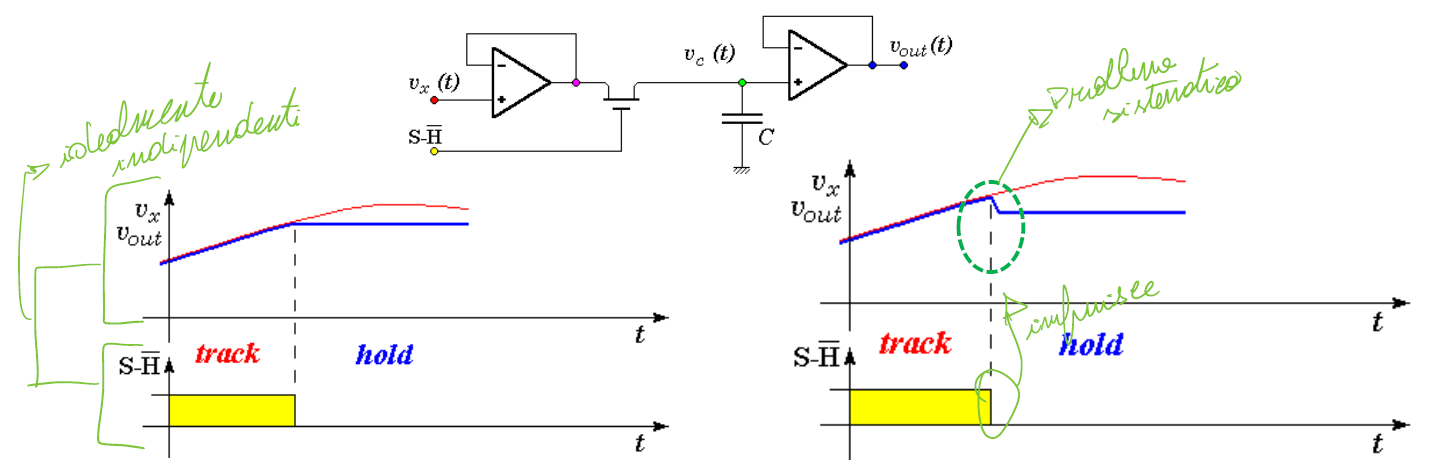
\includegraphics[scale = 0.55]{Tensioni dell'S&H dovuto alla sottrazione di cariche.png}
\end{figure}


L'ampiezza dovuta alla sottrazione di cariche è chiamato hold step o pedestal. \newline

\newpage 

\subsection{Hold step o pedestal} 
\footnote{Slide della prof | SDME 3.Conversione AD e Convertitori - Parte II | pag 25 - 28 \\  
Appunti | 2025-03-25 | pag 8} 

\begin{figure}[h]
    \centering
    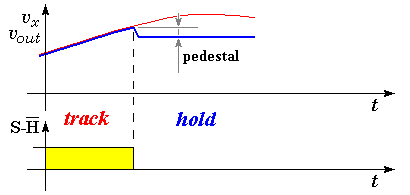
\includegraphics[scale = 1]{Pedestal.png}
\end{figure}

L'hold step o pedestal è determinato dalla non idealità del circuito S \& H perchè tra Gate e Drain del MOS-FET reale sussiste una capacità parassita, 
come si può vedere in figura: 

\begin{figure}[h]
    \centering
    \includegraphics[scale = 1]{Capacità parassita mosfet sample and hold.png}
\end{figure}

Durante la fase di track, la capacità parassita deve essere caricata in questo modo: 
il gate deve essere positivo rispetto al drain, quindi la capacità parassita ha le cariche negative sul lato superiore 
e positive sull'armatura opposta del condensatore C di memoria. \newline 

Il condensatore C di memoria usato nel S \& H ha, ai suoi capi, ha una tensione positiva. \newline 

Nell'istante in cui viene cambiato lo stato del gate e il MOSFET si interdice (cioè idealmente diventa un interruttore aperto), 
la tensione del gate deve diventare negativa rispetto alla tensione del drain. \newline 

Quindi, la capacità parassita deve invertire la polarità: per fare ciò, si carica delle cariche positive del condensatore di memoria C, 
come mostrato in figura: 

\begin{figure}[h]
    \centering
    \includegraphics[scale = 1]{Capacità parassita mosfet sample and hold si carica dal condensatore di memmoria.png}
\end{figure}

Dopo che ciò si è svolto, le cariche positive e negative nei due circuiti si presentano in questa maniera: 

\begin{figure}[h]
    \centering
    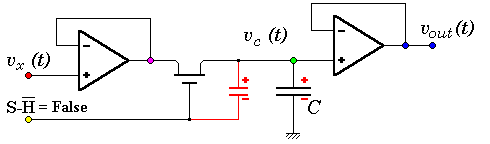
\includegraphics[scale = 1]{Capacità parassita mosfet sample and hold dopo che si è caricato dal condensatore di memmoria.png}
\end{figure}

\newpage

Per ridurre il pedestal, si può: 

\begin{itemize}
    \item mettere un MOSFET con capacità parassita estremamente piccola 
    \item aumentare il valore della capacità di memoria C molto superiore rispetto alla capacità parassita
\end{itemize}

La formula per calcolare il pedestal è la seguente: 

{
    \Large 
    \begin{equation}
        \text{pedestal} = \frac{1}{C}
    \end{equation}
}

dove le dimensioni del pedestal sono i volt. \newline 

Dalla formula si può notare che il pedestal è il reciproco del condensatore C di memoria. \newline 

\newpage 

\subsection{Banda passante} 
\footnote{Slide della prof | SDME 3.Conversione AD e Convertitori - Parte II | pag 29 \\  
Appunti | 2025-03-25 | pag 8} 

Un altro elemento parassita presente in un S \& H reale è una resistenza parassita $R_p$ in serie all'OmAmp e al MOSFET, 
proprio perchè questi due componenti presentano una resistenza idealmente nulla, ma che nella realtà è presente. \newline 

Possiamo rappresentarla con questa nuova resistenza parassita $R_p$: 

\begin{figure}[h]
    \centering
    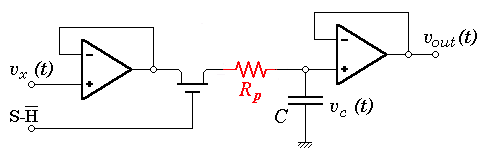
\includegraphics[scale = 1]{Resistenza parassita nell'OpAmp.png}
\end{figure}

Questa $R_p$ è difficile da stimare. \newline 

Facendo uno "zoom" del circuito dopo il Mosfet e prima del secondo OpAmp, 
il circuito sarà proprio una resistenza in serie al condensatore C di memoria: 

\begin{figure}[h]
    \centering
    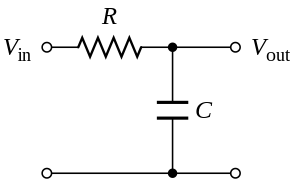
\includegraphics[scale = 0.8]{Filtro passa basso.png}
\end{figure}

Visualizzando il circuito R e C in Fourier, è proprio un filtro passa-basso dove la frequenza di taglio è: 

{
    \Large 
    \begin{equation}
        f_t = \frac{1}{2 \pi RC}
    \end{equation}
}

Se il segnale di ingresso $v_x (t)$ avesse una frequenza superiore rispetto alla frequenza di taglio del filtro passa-basso, 
le sue evoluzioni non si vedrebbero in uscita perchè sarebbero eliminate e / o attenuate dal filtro. \newline 

La banda passante è: 

{
    \Large 
    \begin{equation}
        \text{banda passante} = \frac{1}{C}
    \end{equation}
}

cioè è inversamente proporzionale alla capacità del condensatore di memoria. \newline 

\newpage

\section{Sample and Hold reale e capacità di memoria}
\footnote{Slide della prof | SDME 3.Conversione AD e Convertitori - Parte II | pag 30 \\  
Appunti | 2025-03-25 | pag 9}

Per riassumere, la scelta del valore del condensatore di memoria C del Sample and Hold influisce sui seguenti parametri: 

\begin{figure}[h]
    \centering
    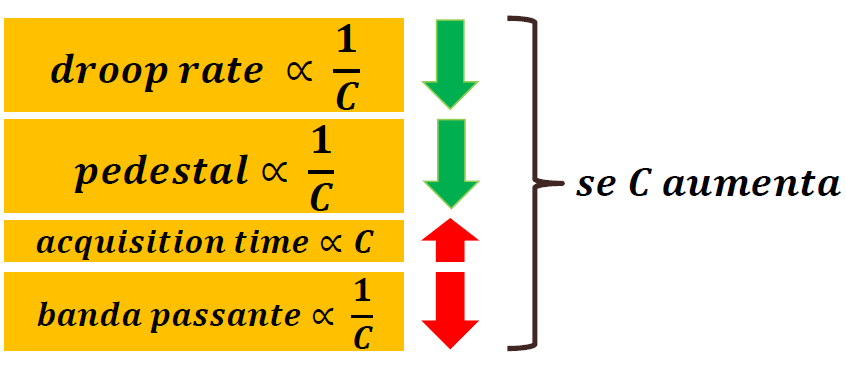
\includegraphics[scale = 0.5]{Valore di C di memoria nel Sample and Hold reale.PNG}
\end{figure}

Il costruttore di S \& H non assume una decisione, ma lascia a noi utilizzatori la scelta della capacità di memoria da collegare, 
che sia più adatta per la nostra specifica applicazione. \newline 

Per aiutarci in questa scelta, il costruttore ci fornisce dei grafici di questi quattro parametri che varieranno in base al valore di C, che rappresentano il comportamento reale del dispositivo. \newline 

\newpage 

